
\section{Introducere}
\hfill

Blockchain-ul poate fi privit ca un registru digital de dimensiuni foarte mari ce este rezistent la manipularea datelor care îl compun. Are un caracter distribuit, lucru evidențiat de lipsa unui spațiu unic în care sunt stocate datele. De asemenea nu conține o singură entitate centrală, încrederea este oferită de procesele ce se desfășoară în interiorul lui, și la care participă, în anumite cazuri, toți utilizatorii din rețea.\\

Caracteristicile tehnologiei oferă posibilitatea unei comunități de utilizatori să efectueze tranzacții și să le înregistreze în blockchain fiind apoi publice și verificabile de către oricine. Odată publicate tranzacțiile nu se pot modifica \cite{Blockchain_Overview_NIST}.\\

Conceptul de blockchain a început să devină din ce în ce mai popular odată cu apariția primei criptomonede numite Bitcoin în 2008. De atunci a început să se pună problema unei forme de stocare a banilor în mod electronic sigur și fără a depinde de o entitate centrală precum o bancă.\\

Vom vedea în capitolul despre algorimii de consens că siguranța și validitatea informațiilor stocate se păstrează datorită implicării multor entități, fiecare având ca scop rezolvarea unor probleme dificile. Dovada muncii lor aduce beneficii de ambele părți pentru că fiecare entitate este răsplătită pentru munca depusă iar informațiile pe care a ales să le publice sunt gata să fie trimise pentru a fi verificate, urmând apoi să fie publicate pentru ca toți participanții să știe.\\

\hfill

\section{Noduri}
\hfill

Putem defini ca nod într-un blockchain orice dispozitiv conectat la rețea și care participă la anumite acțiuni \cite{Blockchain_Node_Types}. Comunicarea dintre noduri se realizează prin rețele de tip Peer-To-Peer, comunicare ce se face constant cu un volum mare de date deoarece toate nodurile trebuie să fie capabile să spună ceva despre conținutul din blockchain.\\

În blockchain-urile populare cum este Bitcoin \cite{Bitcoin} sau Ethereum \cite{Ethereum} putem face o diferențiere între tipurile de noduri bazată pe rolul pe care acestea le au în rețea. Rolurile presupun acțiuni ca stocarea întregii informații din interiorul blockchain-ului, validarea unui nou conținut și înștiințarea celorlalte nodurilor pentru a asigura caracterul distribuit.\\

\begin{enumerate}
    \item \textbf{Full nodes.} \\
    
    Nodurile complete (\textit{full nodes}) sunt nodurile care stochează întreaga informație din blockchain. Le putem privi ca unități de management pentru că acționează ca puncte cheie de care depind celelalte tipuri de noduri.\\
    
    Nodurile complete sunt cele care vor răspunde la noile informații prin verificarea și stocarea lor în propria copie locală.\\
    
    \begin{figure}[H]
    \centering
    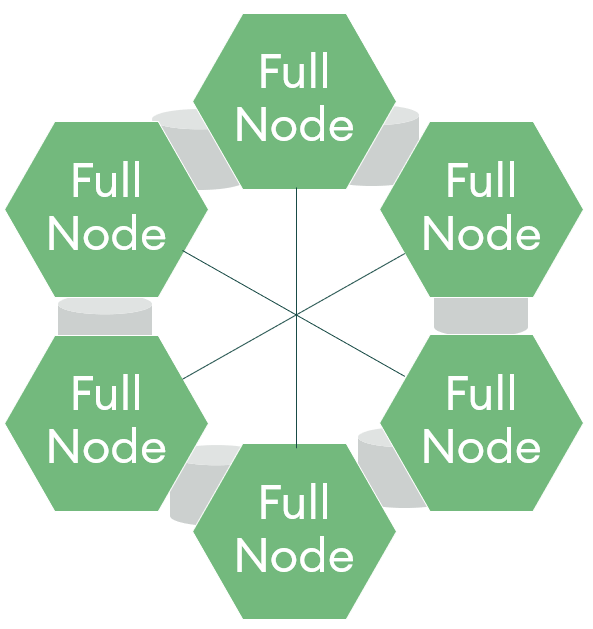
\includegraphics[scale=0.35]{Images/BC_FullNodes.png}
    \caption{Rețea în care sunt legate doar noduri complete - sursă: \cite{Blockchain_Node_Types}}
    \end{figure}
    
    În practică însă nu sunt atât de multe noduri complete. Acest fapt este datorat cantității uriașe ce are nevoie să fie stocată fizic pe fiecare nod. De exemplu rețeaua blockchain Bitcoin are în jur de 10000 de noduri complete iar conținutul a depășit pragul de 300 de gigabytes în septembrie 2019 \cite{Blockchain_Size1} ajungând acum la puțin peste 350 gigabytes de informație \cite{Blockchain_Size2}.\\
    
    Pe lângă rolul de unități de stocare, nodurile complete sunt cele care au autoritate asupra nodurilor secundare de tipuri diferite. Elementele definitorii nodurilor complete sunt validarea semnăturilor din fiecare tranzacție și alegerea noilor tranzacții ce doresc a fi procesate.\\
    
    Vom vedea în secțiunile ce implică validarea unei tranzacții și ce probleme ar putea să apară dacă am omite acest pas.\\
    
    Alegerea noilor tranzacții se reduce la profitul ce poate fi câștigat din urma procesării și publicării lor în registru.\\
    
    Soluția nodurilor complete este favorabilă companiilor ce aleg să investească într-un anumit blockchain pentru a-i spori caracterul descentralizat și pentru a beneficia de răsplata oferită în urma muncii lor.\\
    
    \item \textbf{Light nodes.} \\
    
    Nodurile ușoare sunt nodurile care stochează doar o mică parte din întregul blockchain. Scopul lor este de a păstra doar elemente precum identificatori ai conținutului pentru a putea apoi verifica și accesa tranzacțiile la care fac referire \cite{Blockchain_Node_Types}.\\
     
    Vom vedea în secțiunea despre structură cum acești identificatori ne pot garanta un istoric sigur al proceselor desfășurate pentru ca tranzacțiile să fie acceptate.\\
    
    \begin{figure}[H] 
    \centering
    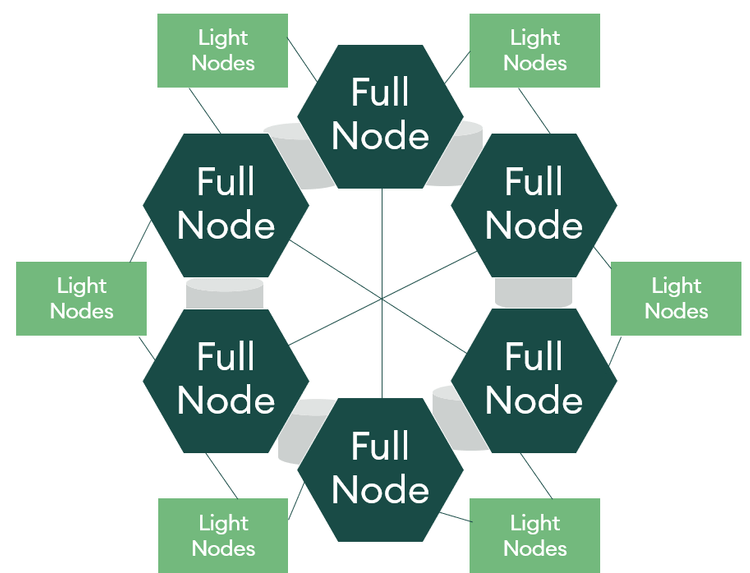
\includegraphics[scale=0.33]{Images/BC_LightNodes.png}
    \caption{Rețea în care noduri ușoare comunică cu noduri complete - sursă: \cite{Blockchain_Node_Types}}
    \end{figure}
    
    Figura 2.2 arată cum nodurile ușoare depind de cele complete numite, în cazul acesta, noduri părinți pentru a-și lua informația de care au nevoie. Securitatea revine nodurilor complete care trebuie să fie capabile să livreze informațiile valide cerute ce nodurile copil.\\
    
    În majoritatea cazurilor nodurile ușoare se găsesc sub forma portofelelor electronice și au rolul de a stoca tranzacțiile și de calcula automat cantitățile de criptomonede avute.\\
    
    \item \textbf{Worker nodes.} \\
    
    Nodurile lucrătoare sunt cele care au nevoie de cea mai multă putere de procesare. Ele sunt cele care vor intra în competiția ce are ca scop rezolvarea unei probleme dificile, a cărei rezultat este definitoriu în pasul de publicare al unui nou conținut în blockchain.\\
    
    Vom vedea mai pe larg în secțiunea despre algorimii de consens de ce această problema se păstrează grea și de ce nodurile lucrătoare rezolvă marea parte din procesele desfășurate în blockchain.\\
    
    Consumul de energie ridicat pentru anumite noduri lucrătoare ce participă la algoritmi de tip Proof of Work au generat cu timpul termenul de minare \cite{Blockchain_Node_Types}. Termenul provide din ideea muncii intense desfășurate ce este răsplătită la final în criptomonede.\\
    
    În practică mai multe noduri lucrătoare comunică cu un nod complet deținut de o companie investitoare care strânge profitul colectiv  și îl împarte după cât a lucrat fiecare. Acest proces a făcut ca minatul criptomonedelor să devină din ce în ce mai popular promovându-se ideea că oricine îl poate realiza de pe orice dispozitiv și poate fi și răsplătit pe măsura muncii lui \cite{Blockchain_Node_Types}.\\
    
    Rolurile celor două tipuri de noduri, complet și muncitor, sunt bine delimitate. Nodul complet este gândit spre a spori gradul de distribuire al conținutului din blockchain stocând o clonă a lui și lucrând atât la verificarea și publicarea informațiilor cât și la extragerea și trimiterea unor noi tranzacții spre a fi procesate. El nu creează însă de fiecare dată informație nouă.\\
    
    Procesele ce stau la baza creării unor noi informații se desfășoară în nodul lucrător și care la final trimite ce a realizat către un nod complet pentru a i se valida munca. Dacă se dovedește a fi corect, nodul lucrător este recompensat.\\
    
    De menționat este și faptul că nodul miner depinde de unul complet însă relația inversă nu este adevărată, un nod complet poate fi creat având nici un miner atașat. În această situație nodul complet poate lua și rolul de miner pe lângă cel de participant la validarea colectivă a informației \cite{Blockchain_Node_Types}.\\
    
    \begin{figure}[H] 
    \centering
    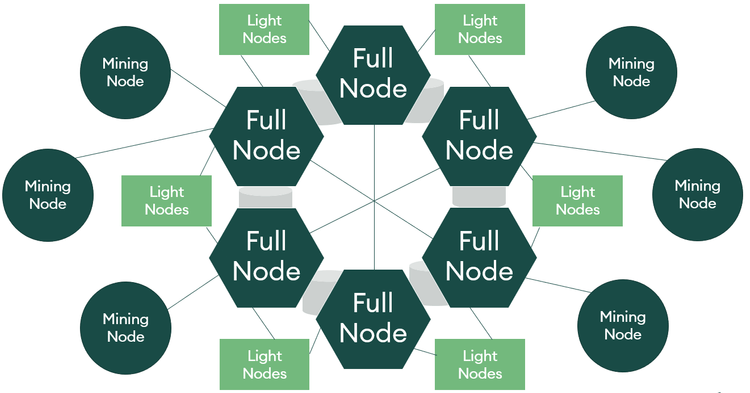
\includegraphics[scale=0.55]{Images/BC_WorkerNodes.png}
    \caption{Rețea în care noduri complete comunică cu ambele subtipuri de noduri - sursă: \cite{Blockchain_Node_Types}}
    \end{figure}
    
\end{enumerate}

\section{Permissionless \& Permissioned}
\hfill

În ceea ce privește o categorisire a blockchain-ului putem distinge două mari categorii: fără permisiune (\textit{permissionless}) și cu permisiune (\textit{permissioned}). În cele fără permisiune oricine poate intra în rețeaua blockchain-ului și poate participa la procesele care se desfășoară în interior. Cele cu permisiune reduc numărul de utilizatori doar la cei aleși pe criterii specifice unui blockchain privat și ridică nevoia unei entități de control care să managerieze întreaga rețea.\\

\begin{enumerate}
    \item \textbf{Permissionless.} \\
    
    Blockchain-urile fără permisiune sunt rețelele la care se poate conecta oricine având și posibilitatea de a publica nou conținut \cite{Blockchain_Overview_NIST}. Pentru acest tip de blockchain adesea se întâlnesc platforme open-source ce permit accesul facil la rețea și ușurează comunicarea cu acestea.\\
    
    Elementele care trebuie să fie mereu disponibile sunt posibilitatea de a citi și adauga nou conținut. Acest lucru poate reprezenta o portiță prin care atacatorii pot introduce date incorecte sau preasamblate pentru a le aduce avantaje materiale. De aceea blockchain-urile permissionless au nevoie de ceea ce se numește algoritm de consens care să dea regulile prin care un nou conținut ajunge să fie salvat în blockchain \cite{Blockchain_Overview_NIST}.\\
    
    Cele mai populare astfel de blockchain-uri sunt Bitcoin și Ethereum, însă există o serie lungă de produse, fiecare concurând cu diferite implementări ce aduc plus eficienței cu care se desfășoară evenimentele.\\
    
    \item \textbf{Permissioned.} \\
    
    Blockchain-urile cu permisiune sunt cele în care există o autoritate care decide ce drepturi și roluri poate avea fiecare membru din rețea \cite{Blockchain_Overview_NIST}. Această autoritate poate lua decizii pe toate planurile din interiorul rețelei, poate restrânge dreptul unor noduri de a vizualiza conținutul din blockchain, poate limita ca doar anumite noduri să poată crea tranzacții sau doar să le verifice și să le publice.\\
    
    Astfel de rețele blockchain pot fi ca și în cazul precedent create și menținute folosind software-uri open-source cum este și cazul BigchainDB, tehnologia descrisă în capitolul următor.\\
    
    Nu trebuie omis faptul că într-un blockchain permissioned se respectă toate evenimentele care se petrec în mod normal în formatul permissionless. Conținutul din blockchain este distribuit și respectă proprietatea că informația nu poate fi alterată. În ceea ce privește algoritmul de consens, el are loc însă nu este la fel de consumator de resurse și putere de procesare datorită faptului că nodurile membre se autentifică pentru participare iar factorii de decizie pentru validarea unui nou conținut pot fi mai relaxați.\\
    
    În cazul acestui tip de blockchain nodurile trebuie să aibă un grad de încredere mai mare, atât între ele cât și față de autoritatea care îi manageriază. Încrederea este cea pe baza căreia se pot reduce etapele complicate și consumatoare de resurse. De asemenea, dacă un nod este considerat malițios, el își poate pierde toate drepturile pe care le are în rețea.\\
    
    De obicei acest tip de blockchain este întâlnit la organizații ce doresc să beneficieze de proprietățile pe care le aduce tehnologia dar în același timp doresc un nivel de control asupra lucrurilor care se petrec \cite{Blockchain_Overview_NIST}. Situațiile pot varia în funcție de ce necesități are fiecare. Se pot, de exemplu, crea blockchain-uri private în care membrii să facă parte din organizații partenere iar tranzacționarea să se facă în acest format electronic. Se pot decide de comun acord obligațiile și drepturile pe care le are fiecare participant și se poate genera un plan prin care se iau deciziile.\\
    
    Am văzut cum blockchain-urile permissioned se pretează unui cadru privat. De aceea nu este obligatorie transparența totală, tranzacțiile se pot procesa și publica în blockchain însă doar cel care tranzacționează și cel căruia îi este destinată tranzacția pot vedea conținutul complet.\\
    
    Cum spuneam, gradul de securitate poate părea mai slab decât al celuilalt tip de blockchain și asta poate atrage mai mulți atacatori însă este mai ușoară detecția proceselor malițioase și a persoanelor din spatele lor datorită nevoii, în anumite cazuri, a autentificarii \cite{Blockchain_Overview_NIST}.\\
    
\end{enumerate}

\clearpage

\section{Elemente criptografice}

Tehnologia blockchain are la bază un cumul de mecanisme și structuri criptografice foarte puternice care asigură securitate și persistență. Printre ele se numără funcțiile hash și sistemele de criptare asimetrice.\\

Funcțiile hash sunt funcții criptografice ce asigură integritatea datelor. Ele sunt capabile să primească un input în teorie de orice dimensiune și să întoarcă un rezultat unic relativ la ce date a primit \cite{Blockchain_Overview_NIST}. Ceea ce le face utile în diferite procese este ușurița cu care pot fi verificate anumite informații primite în rețea. Orice modificare a conținutului de la care se pleacă va genera un cu totul alt rezultat și astfel putem vedea dacă toate părțile componente ale informației au fost primite sau dacă au fost alterate pe parcurs.\\

Aceste funcții respectă 3 proprietăți \cite{Blockchain_Overview_NIST}:
\begin{itemize}
    \item \textbf{Rezistență la preimagine}. 
    Garantează că funcția este one-way adică este dificil să se calculeze valoarea input-ului dat fiind orice valoare hash. În blockchain această proprietate nu este pusă în valoare datorită caracterului transparent al conținutului. Nodurile pot vedea atât tranzacțiile cât și rezultatul obținut prin trecerea lor printr-ul algoritm de hash.
    
    \item \textbf{Rezistență la a doua preimagine}. 
    Proprietatea ne garantează caracterul unic al rezultatului plecând de la o pereche input-output cunoscută. Dificultatea problemei rămâne dar ipoteza se schimbă în cazul acesta și reprezintă găsirea unui nou input astfel încât trecut prin funcția hash să întoarcă aceeași valoare ca al trecerii unui input cunoscut prin aceeași funcție. În cazul blockchain, unde mulțimea input-urilor posibile este colecția totală de tranzacții transmisă, proprietatea este utilă pentru a fi siguri că dacă știm o submulțime și știm codul hash făcut pe baza ei nu există o a doua submulțime care va avea același rezultat.
    
    \item \textbf{Rezistență la coliziuni}. 
    A treia proprietate merge în aceeași direcție cu cea precedentă și spune că este infezabil de găsit o pereche de input-uri care să rezulte în același cod hash. 
\end{itemize}

Fiecare blockchain poate alege să utilizeze o anumită implementare a unor funcții hash. Bitcoin alege să folosească în etape succesive Secure Hash Algorithm \cite{Bitcoin_Protocol}, pe când Ethereum alege Keccak \cite{Ethereum_Protocol}, ambele întorcând un rezultat pe 32 de bytes. Încercarea de a găși o coliziune în oricare din cei doi algoritmi poate depăși chiar și 30 de bilioane de ani și chiar dacă s-ar găsi este puțin probabil ca input-ul găsit să reprezinte o tranzacție validă \cite{Blockchain_Overview_NIST}.\\

\clearpage

Alte ingrediente criptografice folosite în cadrul blockchain sunt numerele folosite doar o singură dată (\textit{numbers only used once - nonce}). Ele se folosesc în cadrul algoritmilor de consens de tip Proof of Work și reprezintă ceea ce se caută în problema consumatoare de energie. Nonce-urile se folosesc alături de alte date în funcții hash pentru a putea genera valori diferite plecând de la același set inițial de elemente. Procesul poate fi rezumat de formula: \textit{hash (date + nonce) = valoare\_hash}.\\

Mecanismele și elementele de criptografie asimetrică sunt cele care lucrează în blockchain pe două planuri, cel al autentificării și cel al dovedirii posesiei. Criptarea folosită este asimetrică iar aceasta implică două chei diferite, una privată și una publică într-o strânsă legătură. Cheia publică este cea care poate fi vizualizată de către oricine fără a se pierde din securitatea relației cu cheia privată \cite{Blockchain_Overview_NIST}. Simplu spus, având o cheie publică nu putem genera cheia privată.\\

În practică pentru criptare se folosește cheia privată, iar cea publică va folosită ulterior la decriptarea din procesul de verificare al tranzacțiilor. O semnătură digitală se realizează pentru fiecare tranzacție și reprezintă criptarea cu cheia privată a conținutului din tranzacție. Un utilizator alege să folosească semnătura pentru a atesta posesia cheii private și implicit a celei publice regăsite în tranzacții precedente.\\

De asemenea, în contextul blockchain-urilor cu permisiune se pot folosi alternative în ceea ce privește generarea și validarea cheilor asimetrice. Se pot folosi servicii precum Active Directory sau Lightweight Directory Access Protocol pentru a prelua certificate sau alte informații ce autentifică și autorizează un utilizator în rețea \cite{Blockchain_Overview_NIST}.\\

Pentru ușurință anumite blockchain-uri se folosesc de adrese în locul cheilor publice complete. Aceste adrese reprezintă șiruri de caractere scurte obținute prin trecerea cheilor publice prin funcții hash \cite{Blockchain_Overview_NIST}. O tranzacție poate astfel avea ca destinar o adresă despre care putem afirma că este unică deoarece este o valoare hash derivat dintr-o cheie unică. Trebuie însă să reținem că din adresă nu putem reconstrui cheia publică și de aceea, în momentul tranzacționării, pentru ca semnătura digitală să poată fi verificată, trebuie să asociem și cheia publică reală.\\ 

\clearpage

\section{Structura}

Pe parcursul tezei a fost menționată ideea de tranzacție. Tranzacțiile sunt elementele prin care se realizează interacțiunea dintre membrii rețelei blockchain.\\

Deși termenul de tranzacție este universal folosit peste orice implementare de blockchain ea poate avea structură diferită de la caz la caz. În momentul în care cineva dorește să creeze o astfel de structură trebuie să țină cont de elementele ei definitorii: adresa transmițătorului, cheia publică a transmițătorului, o semnătură digitală, unul sau mai multe input-uri și unul sau mai multe output-uri \cite{Blockchain_Overview_NIST}.\\

Input-urile reprezintă informațiile ce se doresc a fi transferate. Dovedirea deținerii informației de către transmițător se poate realiza fie prin referențierea unei tranzacții anterioare în care el are rolul de destinatar, fie prin referențierea unei tranzacții prin care informația a fost creată în blockchain. Legătura către evenimente trecute limitează procesele cu acestea dar în același timp le oferă siguranță. Informația unei tranzacții mai vechi nu poate fi schimbată în noul eventiment. De exemplu în cazul criptomonedelor, nu se poate schimba cantitatea de monezi primită. Securitatea este oferită și de semnătura digitală care atestă că cel care transferă informația este cel căruia ii aparține cu adevărat pentru că este posesorul cheii private asociate celei publice din tranzacție.\\

Output-urile sunt identificatori în blockchain precum adrese sau chei publice cărora se dorește a fi transmisă informația sau o anumită parte din ea. Cazul criptomonedelor permite ca mai multe tranzacții să fie folosite ca input-uri și astfel cantitatea totală să fie adunată și transferată către mai mulți destinatari. Valoarea sumată din input-uri nu trebuie obligatoriu să fie egală cu suma output-urilor, însă trebuie să fie mereu mai mare, diferența vom vedea că va juca rol în motivația minerilor din algoritmul de consens Proof of Work (\textit{PoW}) de a o lua și procesa \cite{Blockchain_Overview_IEEE}.\\

\begin{figure}[H] 
\centering
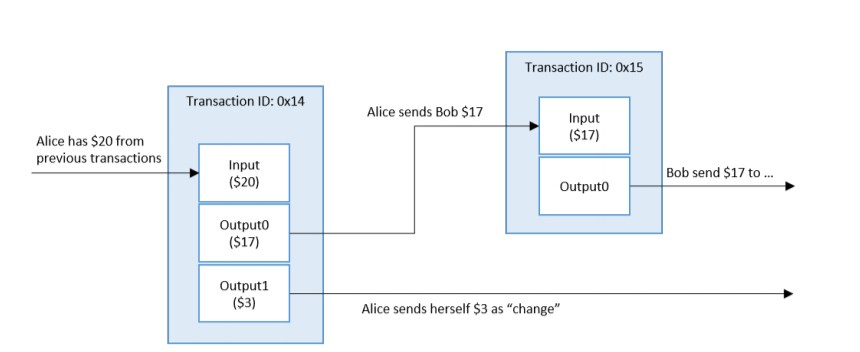
\includegraphics[scale=0.575]{Images/BC_Transaction.png}
\caption{Exemplu de înlănțuire între tranzacții - sursă: \cite{Blockchain_Overview_NIST}}
\end{figure}

Vom vedea că aplicația TrustNews folosește tehnologia descrisă în capitolul următor pentru a putea crea tranzacții ce au ca informații știri luate din diferite surse. Informația este creată și este deținută de nodul care o va prelua.\\

Următoarea și cea mai importantă structura în blockchain este blocul, la care am făcut referire pe parcusul lucrării sub numele de conținut. În momentul în care o tranzacție este efectuată, ea este transmisă în rețea și ajunge în lista fiecărui nod care acum este responsabil să o proceseze sau mai simplu spus să o adauge într-un bloc.\\

Fiecare nod va alege o serie de tranzacții pe care le consideră profitabile și va încerca să creeze structura de bloc compusă din zona de date și zona de metadate (\textit{header}). Datele reprezintă mulțimea de tranzacții alese mai devreme iar metadatele cuprind valori calculate pe baza datelor sau obținute din blocuri precedente.\\

\begin{itemize}
    \item Numărul blocului. Valoare cunoscută și ca înălțimea blockchain-ului reprezintă numărul total de blocuri stocate în lanț.
    \item Versiunea. Face trimitere la setul de reguli folosite pentru validarea conținutului din bloc.
    \item Dimensiunea. Este cantitatea exprimată în bytes a întregului conținut salvat în bloc.
    \item Valoarea hash a blocului precedent. 
    \item Valoarea hash a datelor. Această valoare este dată de rădăcina arborelui Merkle realizată folosind tranzacțiile alese.Procesul implică în prima etapă obținerea codulor hash pentru fiecare tranzacție, apoi mergând către vârf, se obțin codurile hash ale concatenărilor de câte două valori precedent aflate. 
    \item Momentul de timp la care a fost creat blocul
    \item Nonce. Este valoarea unică găsită ca rezultatul problemei dificile din algoritmul PoW și care poate fi omisă dacă blockchain-ul are un alt algoritm de consens.
\end{itemize}

Procesul de înlănțuire este dat de existența în fiecare bloc al codului hash provenit din precedentului bloc. Această valoare hash se realizează având ca date de intrare metadatele blocului precedent. Procesul de hashing ne ajută să determinăm imediat dacă un bloc este format greșit, iar crearea continuă de noi blocuri valide face din ce în ce mai grea munca unui atacator care ar vrea să definească propriile blocuri care i-ar aduce beneficii materiale.\\

\begin{figure}[H] 
\centering
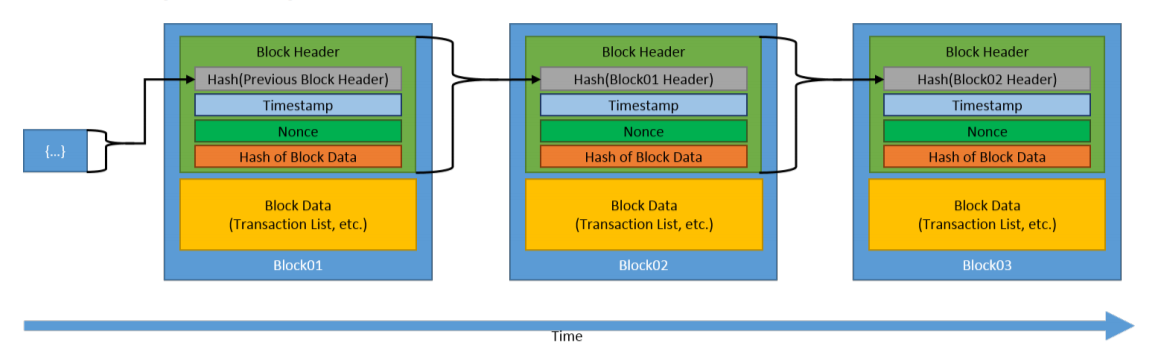
\includegraphics[scale=0.55]{Images/BC_Chaining.png}
\caption{Exemplu de înlănțuire între blocuri - sursă: \cite{Blockchain_Overview_NIST}}
\end{figure}

\section{Algoritmi de consens}

Un factor de decizie foarte important în blockchain este legat de cine are dreptul de a publica noi blocuri și ce reguli trebuie să respecte. Problema alegerii nodului care publică un nou bloc este rezolvată de implementarea unui algoritm de consens.\\

În cazul blockchain-urilor fără permisiune, unde toți participanții pot alege să publice informații, algoritmul poate fi privit ca o competiție având ca rezultat obținerea de beneficiu financiar sub formă de criptomonede \cite{Blockchain_Overview_NIST}. Algoritmul trebuie să fie capabil să gestioneze situații cu mulți participanți care doresc obținerea acelui bonus. În momentul în care un nod creează un nou block, îl trimite în rețea către toți ceilalți participanți pentru a-l valida. Dacă este construit corect, nodul primește răsplata cuvenită.\\

De asemenea algoritmul trebuie să poată decide cine este câștigător atunci când două sau mai multe noduri creează blocuri valide în același timp \cite{Blockchain_Overview_IEEE}. De regulă, în astfel de situații numite \textit{forks}, procesul de creare merge în paralel pe ambele ramuri până când o ramură conține mai multe blocuri decât cealaltă. În acel moment ramura mai lungă se consideră a fi cea principală pentru că a fost mai multă muncă depusă iar cea scurtă este eliminată. Tranzacțiile care au fost adăugate în blocurile de pe ramura eliminată și care nu au fost adăugate în blocuri din ramură câștigătoare se reîntorc în mulțimile fiecărui nod pentru a fi procesate ulterior.\\

De regulă fiecare blockchain are un bloc inițial numit geneză de la care se pornește. Orice nod care acceptă să între în rețea și să participe la algoritmul de consens acceptă implicit validitatea blocului geneză și datorită proceselor de validare poate spune că și blocurile ulterioare au fost construite corect.\\

\clearpage

Fie că vorbim de blockchain-uri cu permisiune fie fără, algoritmul de consens este cel care protejează rețeaua de membrii malițioși care doresc să altereze conținutul. În cazul celor fără permisiune, cel care acționează malițios este oprit de numărul mult mai mare de utilizatori corecți, iar în cazul blockchain-urilor cu permisiune unde numărul nodurilor poate fi redus există acea autoritate de încredere care poate acționa chiar și legal atunci când observă că un utilizator nu respectă regulile la care s-a înscris inițial. Un alt element distinctiv atunci când vorbim de algoritmi de consens pentru cele două tipuri de blockchain-uri este gradul de utilizare al resurselor fizice. În cele cu permisiune adesea se folosesc algoritmi mai relaxați care pot fi reduși doar la simple validări.\\

O formă de algoritm de consens ce a devenit cunoscută odată cu apariția Bitcoin este Proof of Work. În acesta formă, nodul care va publica noul bloc este cel care reușește primul să găsească rezultatul unei probleme criptografice grele dovedind astfel munca depusă. Rezolvarea problemei este dificilă și mare consumatoare de energie dar verificarea rezultatului este ușoară și facilitează procesul de validare de către celalte noduri \cite{Blockchain_Overview_NIST}.\\

Un exemplu de astfel de problemă dificilă este găsirea unei valori hash ce conține pe primele poziții un număr țintă de zerouri. Pentru că procesul de hashing nu întoarce un rezultat previzibil dificultatea este dată de încercarea tuturor posibilităților până la găsirea unui rezultat favorabil. În momentul de față, în Bitcoin, problema se reduce la găsirea valorii nonce astfel încât valoarea hash realizată pe baza metadatelor din bloc să înceapă cu 19 zerouri. Această dificultate este crescută gradual pentru a asigura crearea blocurilor noi odată la aproximativ 10 minute.\\

Dificultatea găsirii acestei valori nonce limitează atacatorii care decid să investească și să dețină o foarte mare parte din puterea de procesare a rețelei pentru a fi singurii care primesc bonusul financiar. Atacul de genul acesta se numește atacul 51\% și implică deținerea a peste jumătate din întreagă putere de procesare a rețelei blockchain. O astfel de putere poate, pe lângă efectul financiar descris anterior, să influențeze conținutul deoarece ar putea valida în mod intenționat un conținut malițios. O abordare al acestui atac implică crearea unui lanț paralel și mai lung decât cel principal în care unele tranzacții pot fi dublate. Când atacatorul decide poate publica ramura creată și, fiind mai lungă, o va înlocui pe cea reală procesată corect. Cu toate acestea, un astfel de atac este nefezabil financiar în momentul de față și devine din ce în ce mai greu de realizat cu cât mai mulți utilizatori aleg să intre în rețea.\\

\clearpage

O altă formă de algoritm de consens este Proof of Stake (\textit{PoS}). Devenită cunoscută odată cu trecerea rețelei Ethereum la versiunea a doua, ea implică un proces similar cu cel al licitațiilor. În blockchain-urile care implementează acest tip de algoritm se presupune că fiecare utilizator are o sumă pe care o poate investi pentru a asigura buna funcționare a întregii rețele. O miză (\textit{stake}) este o sumă pe care un nod este dispus să o dea pentru ca un bloc creat de el să fie publicat. Astfel, nodul câștigător care va publica un nou bloc este cel care oferă miza mai mare \cite{Blockchain_Overview_NIST}.\\

Spre deosebire de PoW, această formă nu implică un consum de resurse intens și din această cauză blockchain-urile care implementează soluția consideră că întreagă cantitate este distribuită și că nu mai este nevoie de o răsplată în urmă procesării blocului. Răsplata financiară în această situație vine din taxele puse pe tranzacții pentru a fi procesate. Pentru că în această formă a algoritmului se poate pune problema unui monopol, există diferite forme prin care se alege cine este cu adevărat cel care publică un block.\\

Forma aleatoare este dată de numărul de noduri aparținând fiecărui utilizator. Un utilizator care deține 30\% din totalul de noduri are 30\% șanse să fie ales, șansă mult mai mare decât cineva ce deține doar 2\% din totalul de noduri. 

Forma prin votare numită și Byzantine Fault Tolerance implică ca software-ul să aleagă un grup de noduri care vor să publice un bloc nou. Odată ales acest grup, membrii participă la mai multe runde de votare asupra cărui bloc este publicat și implicit cine îl va publica \cite{Blockchain_Overview_IEEE}. 

Alte forme pot conține voturi atât în favoarea cât și împotriva anumitor noduri, voturi ce cântăresc mai mult cu cât miza oferită este mai mare. Se creează astfel reputație pentru fiecare nod, reputație pe baza căreia se poate face distincția între un nod corect și unul malițios.\\

\clearpage

\section{Motivație pentru utilizare}

Cu toate că tehnologia blockchain aduce multe beneficii trebuie să ne punem problema dacă ne este cu adevărat utilă. Imaginea din pagina următoare preluată din articolul celor de la National Institute of Standards and Technology (NIST) ne ajută să ne punem întrebările necesare și să determinăm dacă avem nevoie de toate facilitățile pe care le pune la dispoziție blockchain-urile în general.\\

Aplicația TrustNews își propune să stocheze sub formă de blocuri știri preluate de pe platforme publice cunoscute a fi de încredere și are nevoie de proprietățile blockchain.\\

Este nevoie de o zonă distribuită a datelor. Caracterul distribuit ajută la menținerea în siguranță a valorilor introduse corect de noduri cinstite.\\

Aplicația propune existența mai multor noduri care să lucreze atât ca extractori de știri de pe diferite platforme online cât și ca noduri ce publică blocuri.\\

Odată publicate știrile sub formă de tranzacții în blockchain ele nu se mai pot modifica. 
Acest aspect este cel care ne garantează că știrile salvate in TrustNews nu se pot altera pentru a deveni false.\\

Deși software-ul permite, informații sensibile nu vor fi stocate. Conținutul va fi preluat doar din surse publice de media.\\

Pentru că nu vorbim de o soluție clasică ce implică o bază de date în care se gestionează conținutul este nevoie de un algoritm prin care participanții să poată transmite și primi informațiile noi și să le managerieze în propria lor copie a întregului blockchain.\\

În plus, la orice moment, trebuie să existe posibilitatea de a verifica operațiile efectuate și de către cine au fost realizate. Identificarea unui nod ce poate fi echivalat cu un extractor de știri se va face folosind perechile de chei asimetrice generate de un software comun folosit de toți participanții.\\

\begin{figure}[H] 
\centering
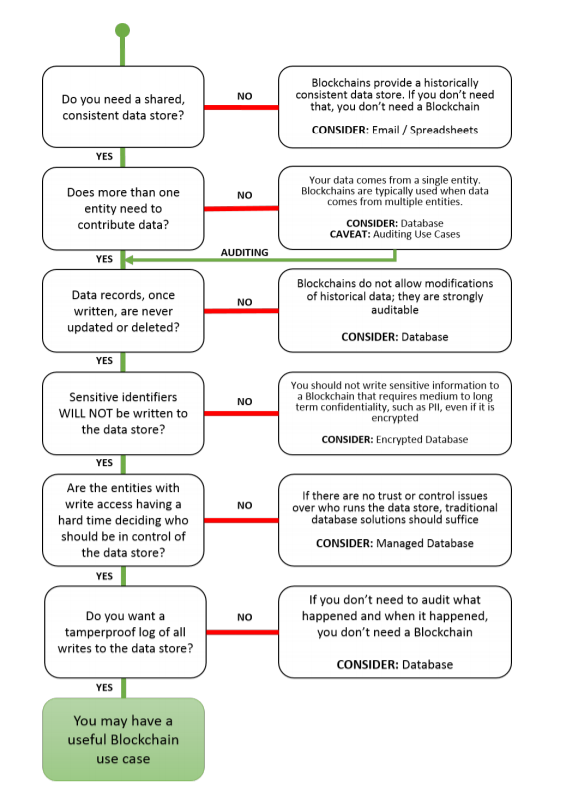
\includegraphics[scale=0.9]{Images/BC_Motivation.png}
\caption{Blockchain Usage Flowchart - sursă: \cite{Blockchain_Overview_NIST}}
\end{figure}

\clearpage